\documentclass{beamer}
%\usepackage{amsfonts,amsmath,oldgerm}
\usepackage{listings}
\usepackage{tcolorbox}
\usepackage{ulem}
\usepackage{algpseudocode}
\usepackage[T1]{fontenc}
\usepackage[utf8]{inputenc}
\usepackage{amsmath}

\usepackage[vlined, linesnumbered]{algorithm2e}

\usepackage{booktabs} 
\usepackage{caption}

\usepackage{tikz}
\usetikzlibrary{shapes.geometric, arrows, positioning}

\tikzstyle{box} = [
    rectangle, 
    minimum width=2.5cm, 
    minimum height=1.2cm, 
    text centered, 
    text width=2.5cm, 
    draw=black, 
    top color=white, 
    thick
]

\tikzstyle{arrow} = [
    ultra thick, 
    ->, 
    >=stealth, 
    gray!80
    %-triangle 60
]

\usetheme{ufrgs}
% \usepackage[sfdefault]{atkinson}

\newcommand{\testcolor}[1]{\colorbox{#1}{\textcolor{#1}{test}}~\texttt{#1}}
\newcommand{\starflet}{\textbf{Star-Fletcher}}
\newcommand{\waveprop}{\texttt{wave\_propagation}}
\newcommand{\waveinsert}{\texttt{wave\_insertion}}
\newcommand{\blockwrite}{\texttt{write\_block}}

% \usefonttheme[onlymath]{serif}

% \useoutertheme{miniframes}
\graphicspath{ {./images/} }
\titlebackground*{rtm}


\newcommand{\hrefcol}[2]{\textcolor{cyan}{\href{#1}{#2}}}

\title{STF, I/O and RTM}
\subtitle{How STF allows trivial overlap of I/O and computations on Forward RTM }
\author{\href{mailto:phbcolle@inf.ufrgs.br}{Pedro Henrique Boniatti Colle}}
\date{Apresentação ERAD/RS -- 07/05/26}

\begin{document}
\maketitle


% Objetivos
% - Introduzir bem os elementos de pesquisa
%   - O que é RTM
%   - O que é STF
% - Como foi a implementação do algoritmo
%   - Segmentação do espaço
%   - Rediscretização do tempo
%   - 1 slide para cada task
% - Resultados Preliminares
% - Conclusão

\section{Introdução}

\begin{frame}{Contexto}
  \begin{itemize}
  \item<+-> \textit{High performance Computing} já é um campo complexo.
  \item<+-> Com o crescimento de IA, há o surgimento de novos aceleradores.
    \begin{itemize}
    \item<+-> CPU
    \item<+-> GPU
    \item<+-> FPGAs
    \item<+-> TPUs
    \item<+-> Hardware Especializado
    \end{itemize}
  \item<+-> Como usar todo o poder de processamento de um parque de alta performance?
  \item<+-> Faz sentido usarmos apenas a GPU nos nodos do parque?
  \item<+-> Porque não todos os recursos?
  \end{itemize}
\end{frame}

\begin{frame}{Sequential Task Flow}
  \begin{itemize}
  \item<+-> \textit{Sequential Task Flow} (STF) é uma técnica de divisão de trabalho em \textbf{tarefas}.
  \item<+-> Essas \textbf{tarefas} podem depender da conclusão de outras tarefas para executar, formando um DAG.
  \item<+-> Elas são submetidas sequencialmente e executam tanto quanto for possível pela ordem de submissão.
  \end{itemize}
  \uncover<4>{
    \centering
    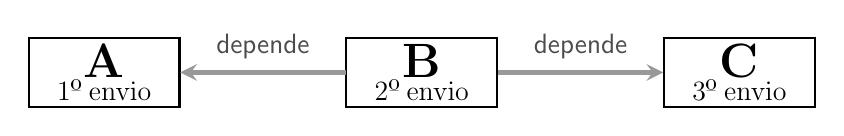
\begin{tikzpicture}[scale=0.7, transform shape]
    
    % Nodes
    \node (B) [box] {\Huge\textbf{B} \\ \Large 2º envio};
    \node (A) [box, left=3cm of B] {\Huge\textbf{A} \\ \Large 1º envio};
    \node (C) [box, right=3cm of B] {\Huge\textbf{C} \\ \Large 3º envio};
    
    % Edges with text
    \draw [arrow] (B.west) -- (A.east) node[midway, sloped, above=0.1cm, font=\Large\sffamily, color=black!70] {depende};
    \draw [arrow] (B.east) -- (C.west) node[midway, sloped, above=0.1cm, font=\Large\sffamily, color=black!70] {depende};
    
    \end{tikzpicture}
  }
\end{frame}

\begin{frame}{Vantagens}
  \begin{itemize}
  \item<+-> Permite a fácil exploração de arquiteturas heterogêneas.
  \item<+-> Faz a gerência automática de dependências.
  \item<+-> Permite a construção de programas de uma forma mais natural.
  \end{itemize}
\end{frame}


\begin{frame}{Atualidade}
  \begin{itemize}
  \item<+-> Há mais de um sistema de STF.
  \item<+-> PaRSEC.
  \item<+-> StarPU
    \begin{itemize}
    \item<+-> Implementa a API diretamente em C.
    \item<+-> Gerência dependências de dado e memória automaticamente.
    \item<+-> Permite vários escalonadores diferentes.
    \end{itemize}
  \end{itemize}
\end{frame}

\begin{frame}{Reverse Time Migration}
  \begin{itemize}
  \item<+-> Qual o nosso objeto de estudo então?
  \item<+-> \textit{Reverse Time Migration} (RTM).
  \item<+-> É uma ferramenta de análise sísmica usada pela indústria petrolífera para encontrar depósitos subsuperficiais de óleo e gás.
  \item<+-> É o principal método de pós-porcessamento das ondas captadas pelos geofones.
  \end{itemize}
\end{frame}

\begin{frame}{Funcionamento}
  \begin{itemize}
  \item<+-> É a discretização de equações diferenciais de onda.
  \item<+-> Trabalha-se com a onda primária e secundária.
  \item<+-> Realiza-se duas etapas:
    \begin{itemize}
    \item<+-> Propaga-se a onda gravada, salvando a cada $k$ passos.
    \item<+-> Lê-se a onda gravada a cada $k$ passos, propagando a onda no sentido contrário ao tempo.
    \end{itemize}
  \item<+-> Esse processo é chamado de \emph{shot} e gera uma imagem subsuperficial parcial.
  \end{itemize}
\end{frame}

\begin{frame}{Paralelismo}
  \begin{itemize}
  \item<+-> Para gerar a imagem final, precisa-se compor vários \emph{shots}.
  \item<+-> RTM é, então, um algoritmo trivialmente paralelizável...
  \item<+-> ... entre shots.
  \item<+-> O paralelismo consiste então em cada nodo computar um \emph{shot}.
  \item<+-> Resultado final é agregado pós-mortem.
  \end{itemize}
\end{frame}

\begin{frame}{Limitações}
  \begin{itemize}
  \item<+-> Os volumes de dados podem ser enormes.
  \item<+-> Um volume de $1024 \times 1024 \times 512$ salvo em ponto fluante de dupla precisão consite em $4Gb$.
  \item<+-> Logo, o processo de salvar a cada $k$ passos e depois ler nessa mesma taxa é muito custoso.
  \item<+-> Diz-se então que RTM é um algoritmo \textbf{I/O bound}.
  \item<+-> Muito esforço tem que vir do programador para gerir essas transfências de dados e maximizar o processamento das máquinas.
  \item<+-> Além disso, com um volume grande o suficiente, computação em um único nodo não é viável.
  \end{itemize}
\end{frame}


\begin{frame}{\starflet}
  \begin{itemize}
  \item<+-> O meu trabalho apresenta \starflet.
  \item<+-> Uma implementação de RTM usando STF em primeira ordem.
    \begin{itemize}
    \item<+-> O espaço é segmentado em blocos.
    \item<+-> Cada tarefa, distribuida aos trabalhadores, é de computar um dos blocos.
    \item<+-> Cada iteração depende das anteriores.
    \item<+-> É possível submeter todas as tarefas enquanto o código executa, sem problemas de sincronização.
    \end{itemize}
  \item<+-> Usou-se o StarPU para essa implementação.
    \item<+-> Uma consequência de usar o STF é que, \textbf{ao modelar o programa em formato de tarefas, naturalmente chegou-se em uma implementação que otimiza I/O}.
  \end{itemize}
\end{frame}


\section{Implementação}

\begin{frame}[fragile]{Implementação}
  \begin{itemize}
  \item<+-> Para esse trabalho utilizou-se o algoritmo \textit{Fletcher}.
  \item<+-> Implementou-se apenas a iteração para a frente no tempo, salvando a cada $k$ passos em disco.
  \end{itemize}

\scriptsize
  \begin{algorithm}[H]
    \SetAlgoLined
\DontPrintSemicolon
\SetKwFunction{FSource}{Source}
\SetKwFunction{FInsert}{InsertSource}
\SetKwFunction{FPropagate}{Propagate}
\SetKwFunction{FSwap}{SwapArrays}
\SetKwFunction{FDump}{WriteVolume}

\SetKwInOut{Input}{Input}
\Input{Ondas $pc, qc, pp, qp$, Iterações totais $st$, Escrita por passos $k$}

\BlankLine
$n \longleftarrow 0$\;
\For{$it \longleftarrow 1$ \KwTo $st$}{
  \FInsert{$pc, qc$}\;
  \tcp{Função Paralela}
    \FPropagate{$pp, pc, qp, qc$}\;
    \FSwap{$pp, pc, qp, qc$}\;
    \If{$n \bmod k = 0$}{
      \FDump{$pc$}\;
      $n \longleftarrow n + 1$
    }
}
  \end{algorithm}


\end{frame}

\begin{frame}{Desafios}
  \begin{itemize}
  \item<+-> Desafios de implementação:
    \begin{enumerate}
    \item<+-> Segmentar em blocos.
    \item<+-> Realizar a comunicação inter-bloco.
    \item<+-> Quebrar a dependência de dados de iterações.
    \item<+-> Rediscretização do espaço das iterações.
    \end{enumerate}
  \end{itemize}
\end{frame}

\begin{frame}[fragile]{Segmentação Espacial}
  \begin{itemize}
  \item<+-> Comunicação inter-bloco adiciona \textit{checks}.
  \item<+-> Utilizou-se a \emph{metaprogramação} para discretizar todos os casos possíveis.
  \item<+-> Dessa forma cada ponto do cubo precisa de apenas 3 operações para determinar quais serão os vários acessos seguintes.
  \end{itemize}

  \lstset{basicstyle=\tiny}
  \onslide<4>
  \begin{lstlisting}[language=python]
def make_cross_comp(d1, d2, lamb):
    p = partial(assignment, d1 = d1, d2 = d2, lamb= lamb)
    return f'''
return ((
    L11 * (
        {p(+1, +1)} - {p(+1, -1)} - {p(-1, +1)} + {p(-1, -1)}
    ) +
    L12 * (
        {p(+1, +2)} - {p(+1, -2)} - {p(-1, +2)} + {p(-1, -2)} + 
        {p(+2, +1)} - {p(+2, -1)} - {p(-2, +1)} + {p(-2, -1)}
    ) +
        ...
    L44 * (
        {p(+4, +4)} - {p(+4, -4)} - {p(-4, +4)} + {p(-4, -4)}
    )) * dinv);
        '''
   \end{lstlisting}
\end{frame}

\begin{frame}{Rediscretização Espacial}
  \begin{itemize}
  \item<+-> Como visto no pseudocódigo, a verão base alterna entre dois buffers.
  \item<+-> Isso segura as execuções e limita quantas tarefas podem ser executadas, criando um ponto de sincronização desnecessário no contexto de tarefas.
  \item<+-> Nisso transformou-se o antigo processo de swap.
    \begin{align*}
       P_c &\leftarrow F(P_p) - P_c \\
       P_c &\;swap\; P_p
    \end{align*}
  \item<+-> Para:
    \begin{align*}
      P_t  &\leftarrow F(P_{t-1}) - P_{t-2} 
    \end{align*}
    
  \end{itemize}
\end{frame}

\section{Resultados Parciais}

\begin{frame}{Resultados}
  \begin{itemize}
  \item<+-> A consequência disso no I/O é:
    \begin{itemize}
    \item<+-> A segmentação espacial reduziu o tamanho de bloco e aumentou o número de operações, permitindo a intercalação da tarefa entre computações.
    \item<+-> A rediscretização fez com que o I/O deixasse de bloquear a execução da iteração seguinte.
    \end{itemize}
  \item<+-> Agora ele pode ser intercalado e a computação não depende do I/O acabar para começar.
  \end{itemize}
\end{frame}

\begin{frame}{Resultados}
    \begin{figure}[ht]
        \centering
            % trim order: Left, Bottom, Right, Top
        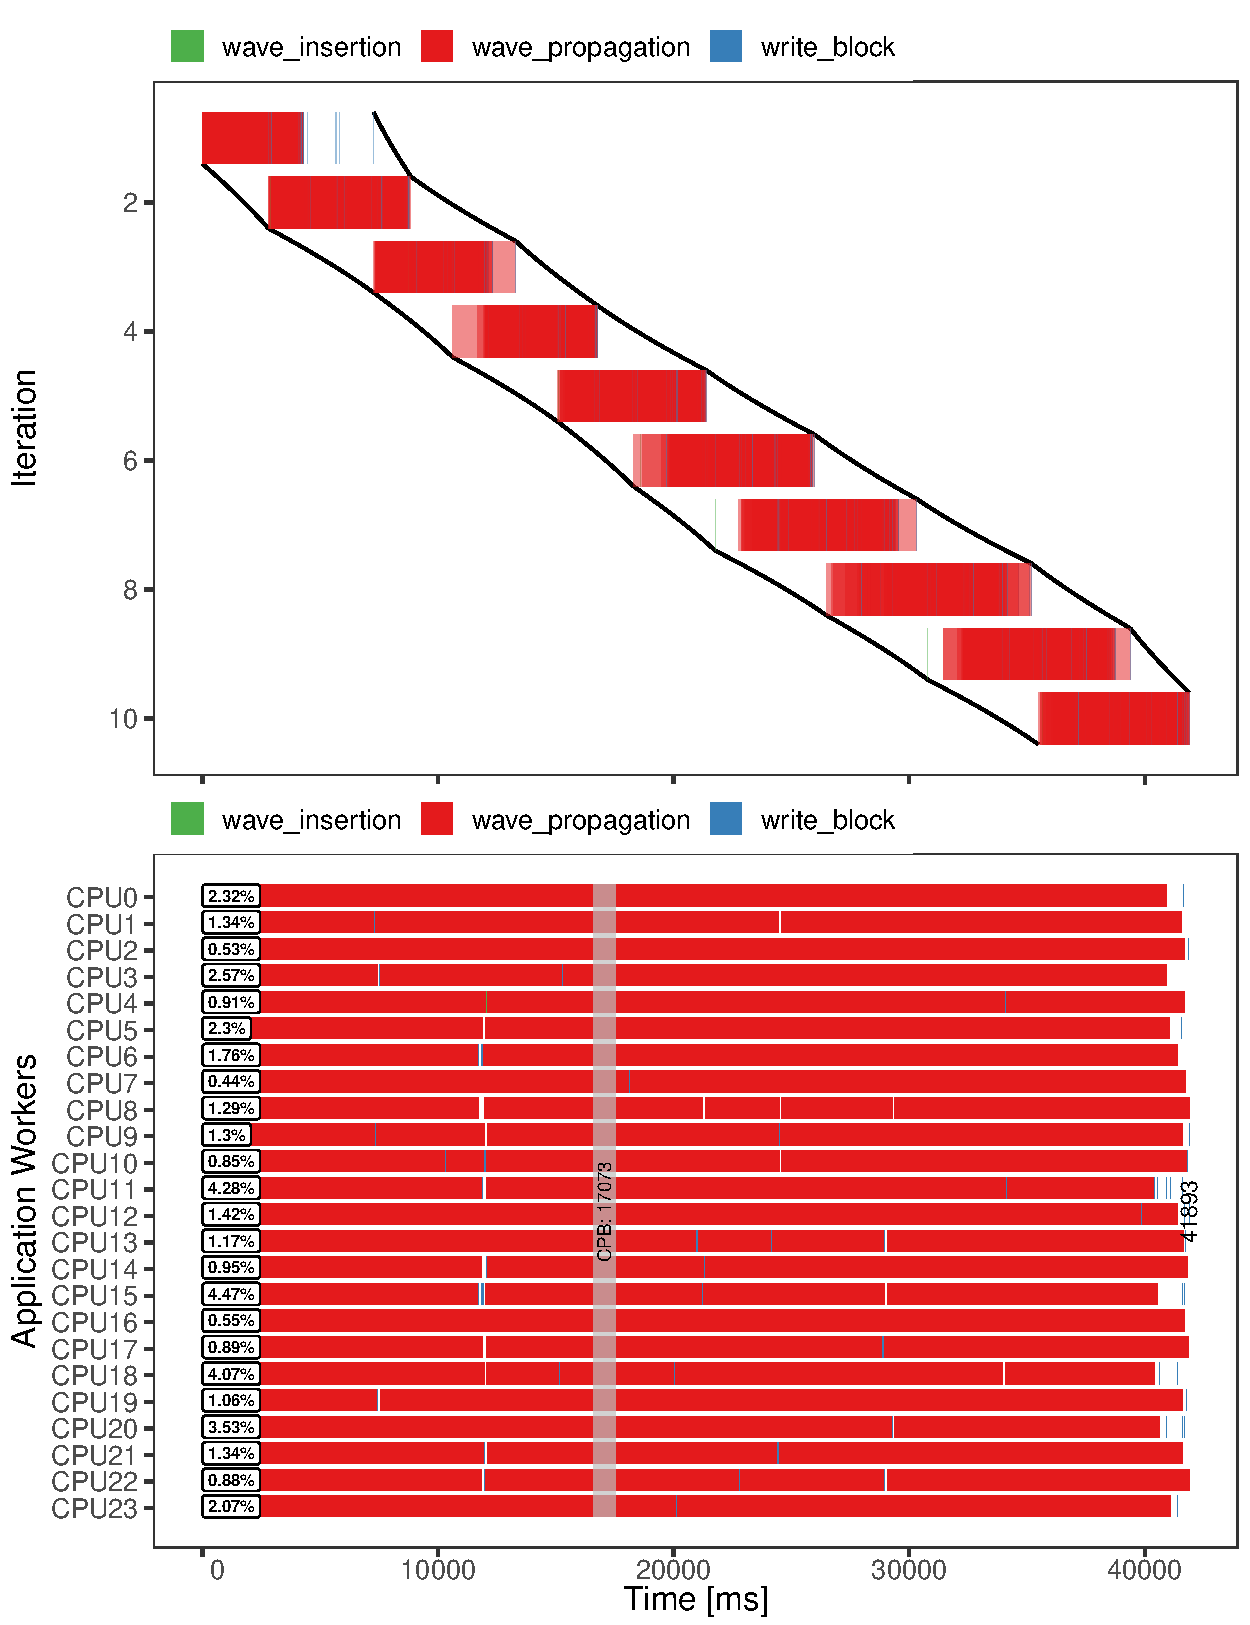
\includegraphics[page=1, trim=0cm 14.38cm 0cm 0cm, clip, width=\textwidth, height=1\textheight]{trace_560_1_4_0_starvz.pdf}
    \end{figure}
\end{frame}

\begin{frame}{Tabela}
    \begin{itemize}
    \item Olhando mais a fundo, temos a tabela.
    \end{itemize}

    \begin{table}[ht]
        \centering
        \caption{Amount of Tasks executed with their Mean, Min and Max execution time in milliseconds.}
        \label{tab:iobench}
        \begin{tabular}{lrrrr}
            \toprule
            Task & Amount & Mean & Min & Max \\
            \waveinsert & 50 & 2.9 & 1.83 & 6.33 \\
            \waveprop & 3200 & 99100 & 55100 & 451000 \\
            \blockwrite & 704 & 39.5 & 13.9 & 628 \\
            \bottomrule
        \end{tabular}
    \end{table}

\end{frame}

\section{Conclusão}

\begin{frame}{Conclusão}
  \begin{itemize}
  \item<+-> O uso do STF foi extremamente útil a implementação do RTM.
    \begin{itemize}
    \item<+-> Os padrões de implementação favorecem essa aplicação \textit{stencil}.
    \item<+-> A necessidade de transferência de dados já uma capacidade provada dos modelos STF, principalmente do StarPU.
    \end{itemize}
  \item<+-> Precisa-se de mais análises comparativas com implementações paralelas convencionais para validar o escopo dos possíveis ganhos de performance.
  \end{itemize}
\end{frame}


\backmatter
\end{document}
